\chapter{Задание}
В лабораторной работе анализируется результат выполнения трех программ. Программы демонстрируют открытие одного и того же файла несколько раз. Реализация, когда файл открывается в одной программе несколько раз выбрана для простоты. Однако, как правило, такая ситуация возможна в системе, когда один и тот же файл несколько раз открывают разные процессы или потоки одного процесса. При выполнении асинхронных процессов такая ситуация является вероятной и ее надо учитывать, чтобы избежать потери данных, получения
неверного результата при выводе данных в файл или чтения данных не в той
последовательности, в какой предполагалось, и в результате при обработке этих данных получения неверного результата. Каждую из приведенных программ надо выполнить в многопоточном варианте: в программах создается дополнительный поток, а работа с открываемым файлом выполняется в потоках.

\section{Первая программа}
Код первой программы приведен на листинге \ref{lst:prog1}
\begin{lstlisting}[label=lst:prog1, caption=Код программы 1, basicstyle=\footnotesize]
#include <stdio.h>
#include <fcntl.h>
#include <pthread.h>
#include <unistd.h>

#define BUFFER_SIZE 20
#define FILE_NAME "alphabet.txt"

void *run(void *arg);

int main()
{
	pthread_t tid1, tid2;
	char buffer_1[BUFFER_SIZE], buffer_2[BUFFER_SIZE];
	int fd = open(FILE_NAME, O_RDONLY);
	
	FILE *fd1 = fdopen(fd, "r");
	setvbuf(fd1, buffer_1, _IOFBF, BUFFER_SIZE);
	
	FILE *fd2 = fdopen(fd, "r");
	setvbuf(fd2, buffer_2, _IOFBF, BUFFER_SIZE);
	
	pthread_create(&tid1, NULL, run, fd1);
	pthread_create(&tid2, NULL, run, fd2);
	
	pthread_join(tid1, NULL);
	pthread_join(tid2, NULL);
	
	close(fd);
	
	return 0;
}

void *run(void *arg)
{
	FILE *fs = arg;
	int flag = 1;
	char c;
	
	while (flag == 1) {
		flag = fscanf(fs, "%c", &c);
		if (flag == 1)
		fprintf(stdout, "%c", c);
	}
	return NULL;
}	
\end{lstlisting}

Результат выполнения программы приведен на рисунке \ref{img:task_1}.
\begin{figure}[H]
	\centering{
		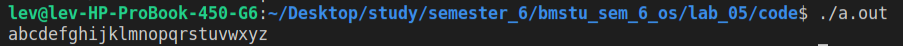
\includegraphics[scale=0.5]{./images/task_1}
		\caption{Результат выполнения программы 1.}
		\label{img:task_1}
	}
\end{figure}

На рисунке \ref{img:prog_1} приведена схема связи структур между собой.
\begin{figure}[H]
	\centering{
		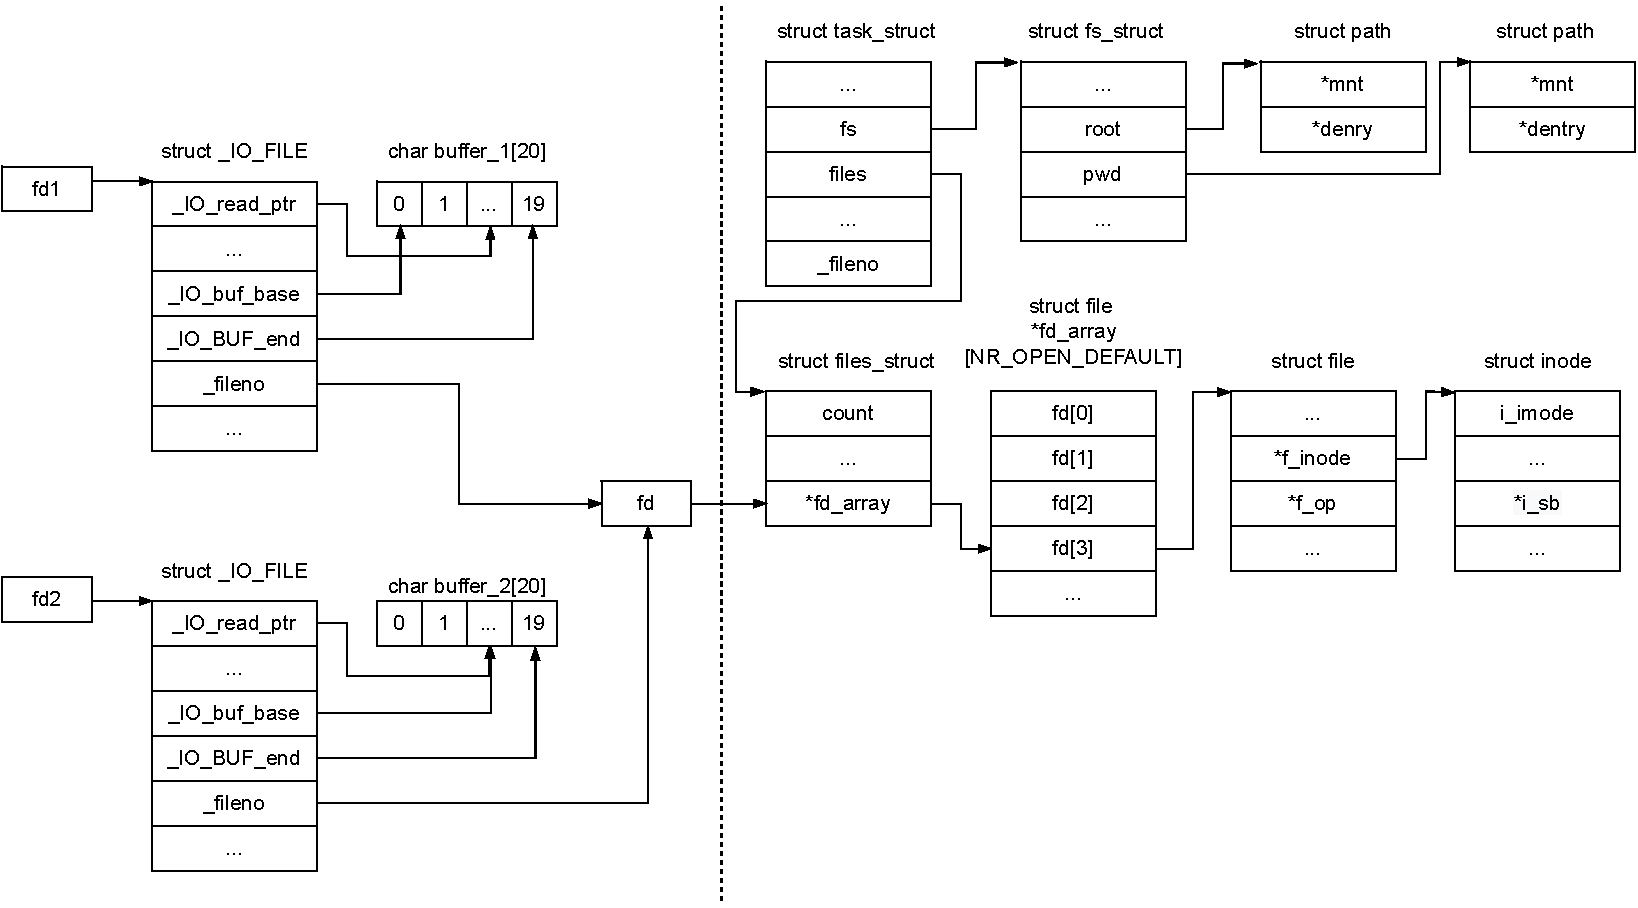
\includegraphics[scale=0.62]{./images/prog_1.pdf}
		\caption{Схема связи структур программы 1.}
		\label{img:prog_1}
	}
\end{figure}

\section{Вторая программа}
Код второй программы приведен на листинге \ref{lst:prog2}
\begin{lstlisting}[label=lst:prog2, caption=Код программы 2, basicstyle=\footnotesize]
#include <unistd.h>
#include <fcntl.h>
#include <pthread.h>
#include <stdio.h>

#define FILE_NAME "alphabet.txt"
pthread_mutex_t lock;

void *run(void *arg);

int main()
{
	char c;
	pthread_t tid1, tid2;
	
	if (pthread_mutex_init(&lock, NULL) != 0) {
		perror("failed mitex init");
		return -1;
	}
	
	int fd1 = open(FILE_NAME, O_RDONLY);
	int fd2 = open(FILE_NAME, O_RDONLY);
	
	pthread_create(&tid1, NULL, run, &fd1);
	pthread_create(&tid2, NULL, run, &fd2);
	
	pthread_join(tid1, NULL);
	pthread_join(tid2, NULL);
	pthread_mutex_destroy(&lock);
	
	close(fd1);
	close(fd2);
	
	return 0;
}

void *run(void *arg)
{
	int fd = *(int*)arg;
	int flag = 1; 
	char c;
	
	pthread_mutex_lock(&lock);
	while (flag == 1){
		flag = read(fd, &c, 1);
		if (flag == 1){
			write(1, &c, 1);
		}
	}
	pthread_mutex_unlock(&lock);
	
	return 0;
}
\end{lstlisting}

Результат выполнения программы приведен на рисунке \ref{img:task_2}.
\begin{figure}[H]
	\centering{
		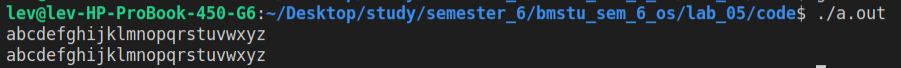
\includegraphics[scale=0.5]{./images/task_2}
		\caption{Результат выполнения программы 2.}
		\label{img:task_2}
	}
\end{figure}

На рисунке \ref{img:prog_2} приведена схема связи структур между собой.
\begin{figure}[H]
	\centering{
		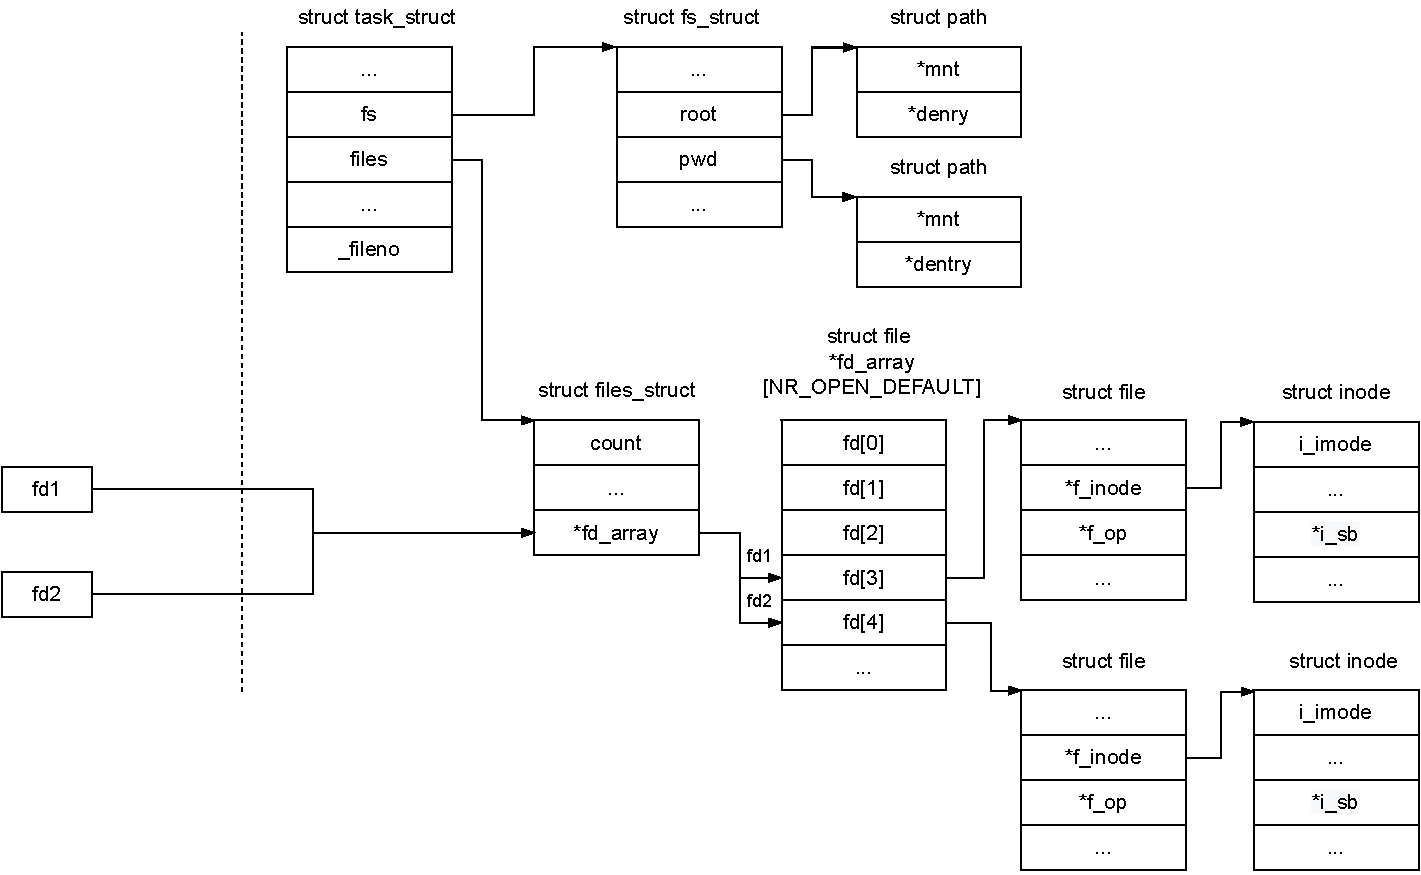
\includegraphics[scale=0.62]{./images/prog_2.pdf}
		\caption{Схема связи структур программы 2.}
		\label{img:prog_2}
	}
\end{figure}

\section{Третья программа}
Код третьей программы приведен на листинге \ref{lst:prog3}
\begin{lstlisting}[label=lst:prog3, caption=Код программы 3, basicstyle=\footnotesize]
#include <fcntl.h>
#include <unistd.h>
#include <stdio.h>
#include <pthread.h>
#include <sys/stat.h>

#define FILE_NAME "alphabet_2.txt"

void *run_1(void *arg);

int main()
{
	struct stat stat_buf_open, stat_buf_close;
	pthread_t tid1;
	FILE *fd1 = fopen(FILE_NAME, "w");
	FILE *fd2 = fopen(FILE_NAME, "w");
	
	lstat(FILE_NAME, &stat_buf_open);
	printf("open_file: inode=%lu, size=%lu\n", stat_buf_open.st_ino, stat_buf_open.st_size);
	
	pthread_create(&tid1, NULL, run_1, fd1);
	
	for (char c = 'b'; c <= 'z'; c += 2){
		fprintf(fd2, "%c", c);
	}
	
	pthread_join(tid1, NULL);
	
	fclose(fd1);
	fclose(fd2);
	
	lstat(FILE_NAME, &stat_buf_close);
	printf("close_file: inode=%lu, size=%lu\n", stat_buf_close.st_ino, stat_buf_close.st_size);
	
	return 0;
}

void *run_1(void *arg)
{
	FILE *fd1 = arg;
	for (char c = 'a'; c <= 'z'; c += 2){
		fprintf(fd1, "%c", c);
	}
	
	return 0;
}
\end{lstlisting}

Результат выполнения программы приведен на рисунке \ref{img:task_3}.
\begin{figure}[H]
	\centering{
		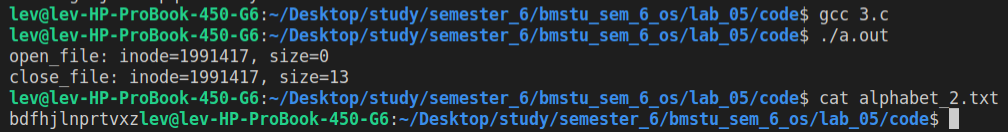
\includegraphics[scale=0.45]{./images/task_3}
		\caption{Результат выполнения программы 3.}
		\label{img:task_3}
	}
\end{figure}

На рисунке \ref{img:prog_3} приведена схема связи структур между собой.
\begin{figure}[H]
	\centering{
		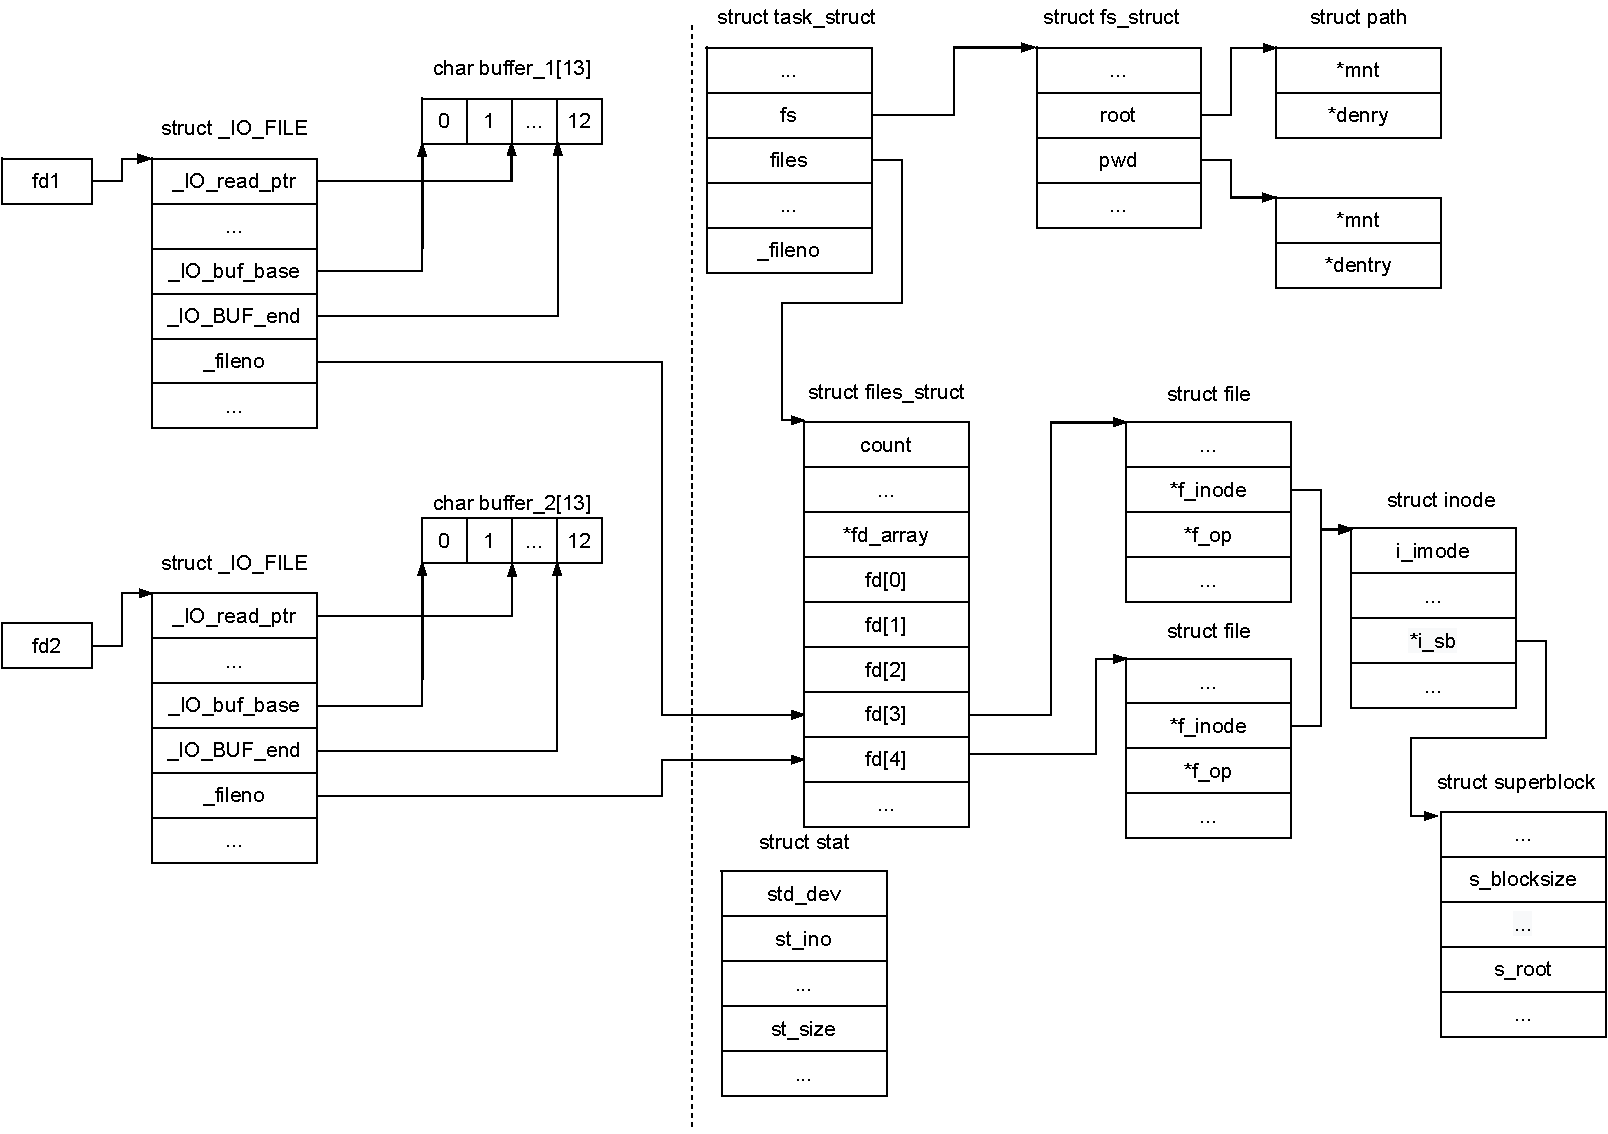
\includegraphics[scale=0.62]{./images/prog_3.pdf}
		\caption{Схема связи структур программы 3.}
		\label{img:prog_3}
	}
\end{figure}

\section{Анализ}
При открытии файла с помощью системного вызова open() в режиме добавления (O\_APPEND) (или fopen(path, "a")) перед каждым вызовом write() смещение в файле устанавливается в конец этого файла, как, например, при выполнении вызова lseek(2).

Системный вызов open() назначает свободный файловый дескриптор для открытого файла в системной таблице открытых файлов. 

При выполнении записи в файл сначала информация записывается в буфер, затем выгружается в файл. При чтении из файла информация также записывает сначала в буфер. Содержание буфера выгружается в файл в трех случаях: когда буфер переполнен, при вызове fclose() и fflush(). 

Одновременный доступ разных процессов к одному и тому же файлу может быть источником проблем -- race condition.

